В общем случае, чтобы решать задачу, нам надо её поставить. И первое чему должен научиться человек, который занимается машинным обучением, статистикой или управлением командой - это ставить задачу. Давайте ставить задачу машинного обучения корректно.


Что такое supervised?

Давайте предположим, что таргета у нас нет, а есть только данные, которые описаны какими-то признаками.

Можем ли мы сделать что-то с этими данными? Мы можем взять наши данные и даже не имея никакого таргета попытаться из них вытащить какое-то знание: построить какие-то картинки и зависимости, попроверять на
них гипотезы, попытаться поделить их на группы. То есть мы можем извлечь знание из данных даже не имея
целевой величины, которую нам надо предсказывать. Например: найти внутреннюю структуру в данных. Есть
отличие между supervised и unsupervised режимах (обучение с учителем и обучение без учителя) - наличие
или отсутствие соответственно таргетов.


Далее мы будем говорить об обучении с учителем. У нас есть некоторая выборка, и она состоит из объектов
и их признаков, и каких-то целевых значений, которые им соответствуют.

\Def Training set $\mathcal{L} = \{ x_i, y_i \}_{i=1}^{n}$ ($x$-- признак, $y$ -- таргет), где

\begin{itemize}
    \item $(x \in \R^p, y \in \R)$ для регрессии
    \item $x_i \in \R^p, y_i \in \{ 0, 1 \}$ для бинарной классификации
    \item $x_i \in \R^p, y_i \in \{ c_1, \ldots, c_n \}$ для многоклассовой классификации
\end{itemize}

Если мы говорим про регрессию, то  почему, если мы можем предсказать 10 чисел, то у нас таргет может лежать именно в одномерном множестве действительных чисел? Что такое число - это точка на числовой прямой. Что такое точка в 10-мерном
пространстве - это радиус-вектор, описывающийся 10 числами. Так что да, мы можем предсказывать хоть 10
чисел одновременно и тогда предсказываемый таргет будет из $\mathbb{R}^{10}$. Например: цвет - чтобы его точно предсказать, надо будет предсказать сразу три канала R, G, B, а не один, так как если по отдельности предсказывать
каждый канал, то у вас нужный цвет не получится ну никак.


Далее для постановки задачи машинного обучения должна быть модель $f(x)$, которая предсказывает для
каждого объекта какую-то величину. И конечно же, нужна функция потерь $Q(x, y, f)$, которую мы используем
чтобы оценить, какая модель лучше работает на наших данных. \textbf{Пока вы не знаете как мерить качество в вашей
задаче, вы её не поставили и вы не знаете как её решать.} Очень часто люди в стартапах и индустрии говорят
нам нужна в первую очередь выборка, так вот пока вы не знаете как будет у вас выглядеть функция потерь и какая будет гипотеза, вам не надо собирать выборку. Потому что в таком случае вы не понимаете какую
задачу вы решаете, и пока вы задачу доформулируете, ваши ожидания к данным могут измениться.

Где мы будем минимизировать функцию потерь?


Выборку мы уже собрали и ничего сделать с ней не можем, $x, y$ - зафиксированны. Модель $f$ скорее всего зависит от каких то параметров, поэтому минимизировать мы будем по параметрам модели, или хотя бы найти
оптимальную функцию $f$, если их какое-то семейство.

\subsubsection*{Примеры задач регрессии и классификации по имеющимся точкам в пространстве признаков:}

Проводим по точкам прямую, наиболее хорошо фитирующую точки

\begin{center}
    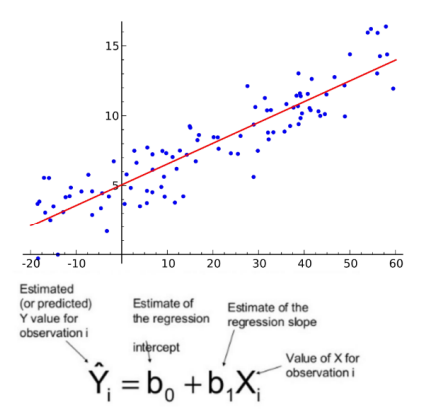
\includegraphics[scale=0.7]{reg.png}
\end{center}


Проводим гиперплоскость, наиболее хорошо разделяющую все объекты на 2 класса

\begin{center}
    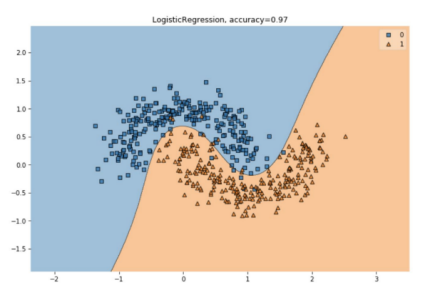
\includegraphics[scale=0.7]{images/classify.png}
\end{center}

